\section{Deadlock prevention}
\subsection{Determine which lock request will be granted, blocked or aborted by the lock manager 1 (LM1)}\label{deadlockLM1section}

\begin{figure}[H]
\centering
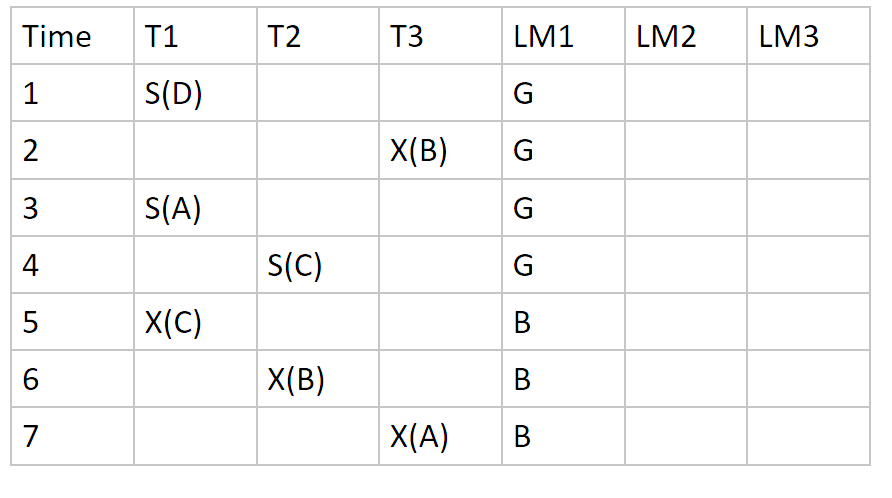
\includegraphics[width=0.7\linewidth]{Lm1TableDeadLockPrevention}
\caption[Table showing how LM1 is handling locks]{Table showing how LM1 is handling lock requests.}
\label{fig:Lm1TableDeadlock}
\end{figure}
\pagebreak
\subsection{Give the wait-for graph for the lock request in the table (Figur \ref{fig:Lm1TableDeadlock}). Give one reason why LM1 Results in a deadlock }

Since the graph (Figur \ref{fig:waitForGraphForLM1DeadLock}) contains a cycle in such a way that T1, T2, T3 is waiting for each other, this results in a deadlock

\begin{figure} [H]
\centering
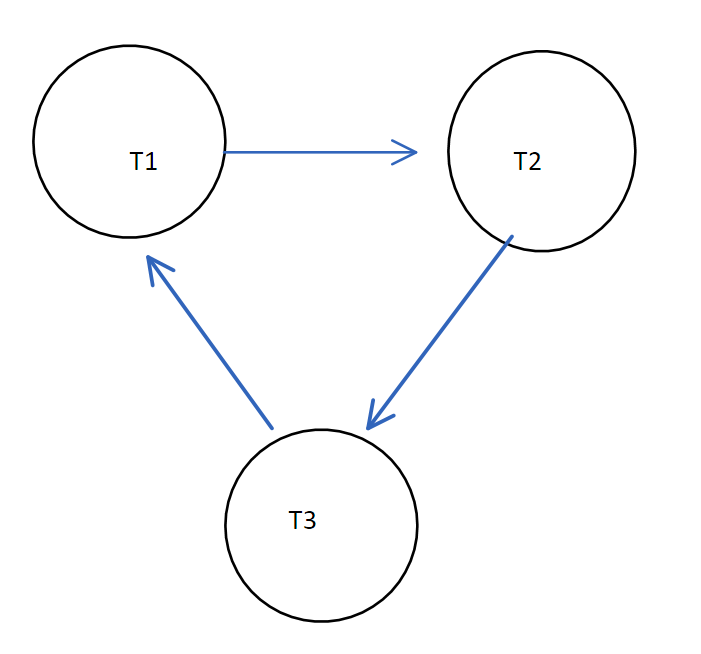
\includegraphics[width=0.7\linewidth]{waitForGraphForLM1DeadLock}
\caption[Wait-for graph of LM1 depicting a deadlock.]{}
\caption{}
\label{fig:waitForGraphForLM1DeadLock}
\end{figure}

	
\pagebreak
\subsection{Deadlock prevention with LM2} \label{deadlockLM2section}
Please note that we have created a table (Figur \ref{fig:Lm123TableDeadlockPrevention}) that illustrates the task of section \ref{deadlockLM2section} and section \ref{deadlockLM3section}.
\begin{itemize}
	\item{\textbf{LM2 with Wait-Die policy.}}
	\item S(D) on T1 is granted.
	\item X(B) on T3 is granted
	\item S(A) on T1 is granted
	\item S(C) on T2 is granted
	\item X(C) on T1 is blocked
	\item X(B) on T2 is blocked
	\item X(A) on T3 is aborted
\end{itemize}

\subsection{Deadlock prevention with LM3} \label{deadlockLM3section}

\begin{itemize}
	\item{\textbf{LM2 with Wound-wait policy.}}
	\item S(D) on T1 is granted.
	\item X(B) on T3 is granted
	\item S(A) on T1 is granted
	\item S(C) on T2 is granted
	\item Abort S(C) on T2
	\item Abort X(B) on T3
	\item X(A) on T3 is blocked
\end{itemize}
\pagebreak
\paragraph{Table depicting lock requst handling of LM1, LM2 and LM3}
The table (Figur: \ref{fig:Lm123TableDeadlockPrevention}) presentates how LM1, LM2 and LM3 handle locks differently. This table is created from the information based on section \ref{deadlockLM1section}, section \ref{deadlockLM2section} and section \ref{deadlockLM3section}.
\begin{figure}[H]
\centering
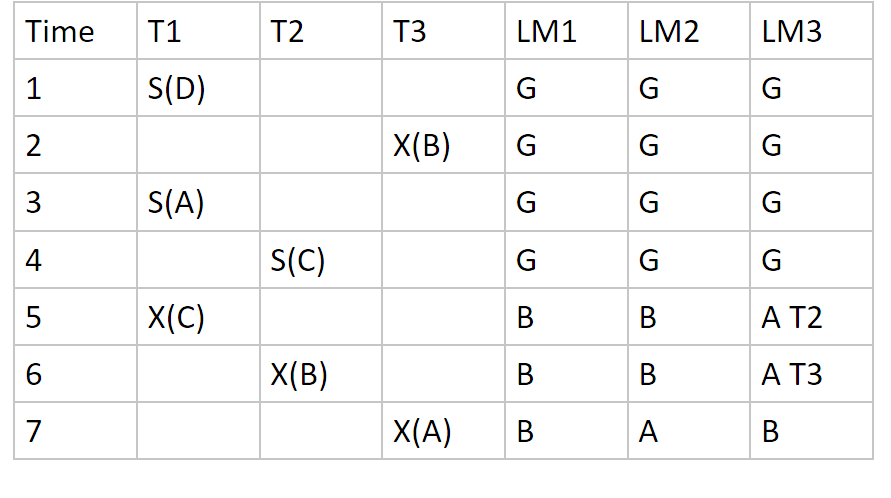
\includegraphics[width=0.7\linewidth]{Lm123TableDeadlockPrevention}
\caption{This is table is a visualization on LM1, LM2 and LM3.}
\label{fig:Lm123TableDeadlockPrevention}
\end{figure}
